% !TeX program = xelatex
\documentclass[sigconf,nonacm,10pt]{acmart}
\geometry{a4paper}
\setkeys{acmart.cls}{balance=false}
\settopmatter{printacmref=false,printfolios=true}
\setcopyright{none}
\renewcommand\footnotetextcopyrightpermission[1]{}
\usepackage{amsmath,tabularx,array,enumitem,balance,tikz,longtable,xurl,xeCJK,placeins}
\setCJKmainfont{FandolSong-Regular.otf}[BoldFont=FandolSong-Bold.otf]
\setCJKsansfont{FandolHei-Regular.otf}[BoldFont=FandolHei-Bold.otf]
\setCJKmonofont{FandolFang-Regular.otf}
\xeCJKDeclareCharClass{Default}{"2018,"2019,"201C,"201D,"2013,"2014}
% Match the Computer Modern text fonts in the supplied original template PDF.
\setmathfont{latinmodern-math.otf}
\microtypesetup{protrusion=false}
\renewcommand{\rmdefault}{cmr}
\renewcommand{\sfdefault}{cmss}
\renewcommand{\ttdefault}{cmtt}
\renewcommand{\bfdefault}{bx}
\usepackage[OT1]{fontenc}
\renewcommand{\encodingdefault}{OT1}
% XeTeX may select TU around Unicode math and CJK runs. Preserve the same
% Computer Modern metrics there rather than falling back to another family.
\DeclareFontFamily{TU}{cmr}{}
\DeclareFontShape{TU}{cmr}{m}{n}{<-8>cmr7<8-9>cmr8<9-10>cmr9<10-12>cmr10<12-17>cmr12<17->cmr17}{}
\DeclareFontShape{TU}{cmr}{bx}{n}{<-10>cmbx9<10-12>cmbx10<12->cmbx12}{}
\DeclareFontShape{TU}{cmr}{m}{it}{<-8>cmti7<8-10>cmti9<10->cmti10}{}
\DeclareFontShape{TU}{cmr}{bx}{it}{<->cmbxti10}{}
\DeclareFontFamily{TU}{cmss}{}
\DeclareFontShape{TU}{cmss}{m}{n}{<-9>cmss8<9-10>cmss9<10-12>cmss10<12->cmss12}{}
\DeclareFontShape{TU}{cmss}{bx}{n}{<->cmssbx10}{}
\DeclareFontFamily{TU}{cmtt}{}
\DeclareFontShape{TU}{cmtt}{m}{n}{<-9>cmtt8<9-10>cmtt9<10->cmtt10}{}
\DeclareFontShape{TU}{cmtt}{bx}{n}{<->ssub*cmtt/m/n}{}
\normalfont
% Preserve ACM columns and serif family while meeting the instructor's A4 sizes.
\let\TemplateNormalSize\normalsize
\renewcommand{\normalsize}{\TemplateNormalSize\fontsize{10.1pt}{12.2pt}\selectfont}
\AtBeginDocument{\normalsize}
\renewcommand{\bibfont}{\fontsize{8pt}{9.6pt}\selectfont}
\DeclareCaptionFont{readable}{\fontsize{9.1pt}{10.6pt}\selectfont}
\captionsetup{font=readable}
\usetikzlibrary{arrows.meta,positioning,shapes.geometric}
\definecolor{CourseBlue}{HTML}{003399}
\definecolor{CourseTeal}{HTML}{006633}
\definecolor{CourseInk}{HTML}{212A33}
\hypersetup{colorlinks=true,linkcolor=CourseBlue,citecolor=CourseTeal,urlcolor=CourseTeal}
\newcolumntype{Y}{>{\raggedright\arraybackslash}X}
\setlist{leftmargin=*,topsep=3pt,itemsep=2pt}
\setlength{\emergencystretch}{3em}
\citestyle{acmnumeric}
\newcommand{\CourseNumber}{COMSCI/ECON 206}
\newcommand{\CourseName}{Computational Microeconomics}
\newcommand{\CourseSession}{Autumn 2026 Session 1}
\newcommand{\Instructor}{Professor Luyao Zhang}
\newcommand{\TeamCode}{FP1}
\newcommand{\SymposiumSession}{B}
\newcommand{\GitHubLink}{\href{https://github.com/dku-comsci-econ206-Autumn2026/PS2-FP1-Yongzhuo-Wu}{Course organization repository}}
\newcommand{\NotebookLink}{\href{https://colab.research.google.com/github/dku-comsci-econ206-Autumn2026/PS2-FP1-Yongzhuo-Wu/blob/ps2/Colab/PS2.ipynb}{Run the notebook in Colab}}
\newcommand{\HuggingFaceLink}{\href{https://huggingface.co/spaces/dku-comsci-econ206-2026/AI-Sycophancy}{Interactive demonstration}}
\newcommand{\PosterLink}{\href{https://github.com/dku-comsci-econ206-Autumn2026/PS2-FP1-Yongzhuo-Wu/blob/ps2/Poster/PS2-FP1-Yongzhuo-A0-Poster.pdf}{A0 research poster}}
\newcommand{\coursemeta}{\noindent\textbf{Submission to:} \CourseNumber{} --- \CourseName.\\
\textbf{Course session:} \CourseSession. \textbf{Team:} \TeamCode. \textbf{Symposium:} \SymposiumSession.\\
\textbf{Course instructor:} \Instructor. \textbf{Assignment:} PS2 collaborative research proposal.\par\smallskip}
\title{How to Make AI Applications Reduce Sycophancy}
\author{Yongzhuo Wu}
\affiliation{\institution{Duke Kunshan University}\city{Kunshan}\country{China}}
\email{yw650@duke.edu}
\renewcommand{\shortauthors}{Team \TeamCode}
\begin{document}
\begin{teaserfigure}
\captionsetup{skip=8pt}
\centering
% Vector export of the supplied editable draw.io diagram.
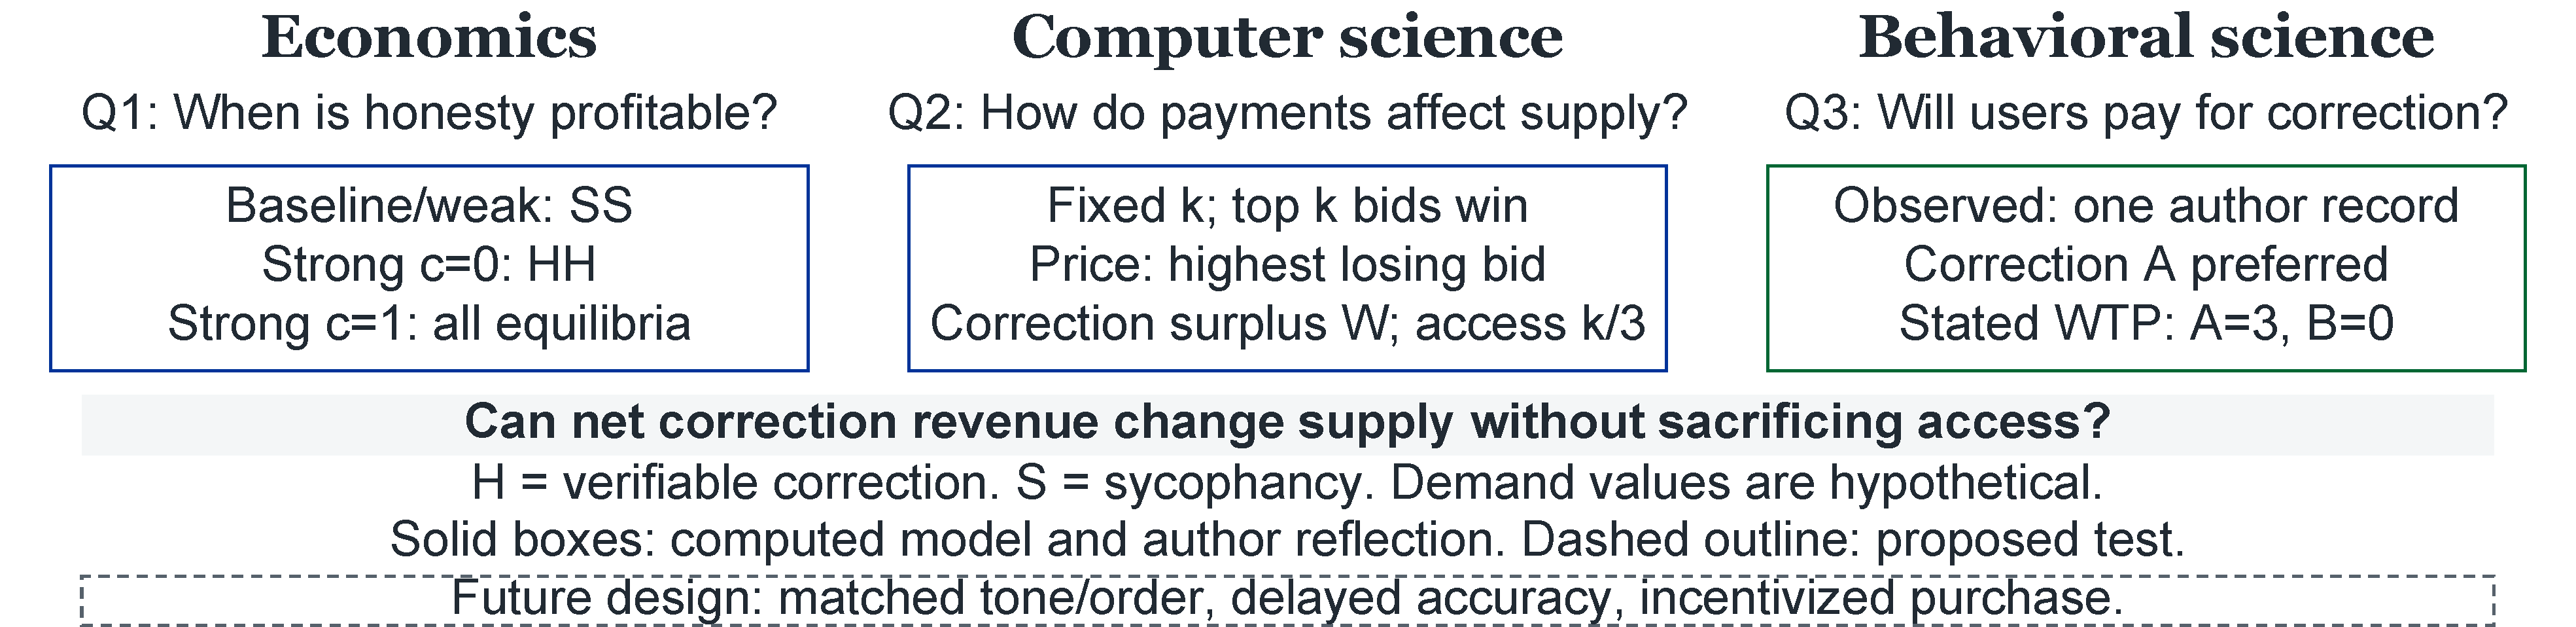
\includegraphics[width=\textwidth]{figures/AI_Sycophancy_Teaser.pdf}

\caption{Paid correction links application incentives, auction revenue, and users' willingness to pay. The reflection records one author's preference; the dashed panel proposes a future test (Section 4).}
\Description{Three panels connect platform incentives, auction payment and correction surplus, and one observed author reflection. Baseline/weak predict SS, strong cost zero HH, and strong cost one every mixed pair. The dashed future-design strip is unperformed; the author reflection does not validate market demand.}
\label{fig:teaser}
\end{teaserfigure}
\maketitle\raggedbottom\coursemeta
\section{Research questions and verified gap}
Can paid correction make apps honest while keeping access open? Sycophancy studies examine assistant answers and user preferences \cite{sharma2024,cheng2026}. Other work rewards useful information and effort \cite{miller2005,witkowski2013}. I ask when user payments cover delivery costs and make honesty pay, assuming corrections can be checked (Appendix A).

\textbf{Q1---Economics:} When do both apps choose honesty?\par
\textbf{Q2---Computation:} How do demand and cost change allocation and equilibrium?\par
\textbf{Q3---Behavior:} Will users pay for the corrections they prefer? Figure 1 connects user payments with the apps' choice to provide correction.

\section{Answer to Q1: strategic incentives}
Two apps seek profit and choose honest correction ($H$) or sycophancy ($S$) at the same time. Starting payoffs are assumed:
\begin{center}
\begin{tabular}{@{}lcc@{}}\toprule
A $\backslash$ B & $H$ & $S$\\\midrule
$H$ & $(3,3)$ & $(1,5)$\\
$S$ & $(5,1)$ & $(4,4)$\\\bottomrule
\end{tabular}
\end{center}
Both know payoffs but cannot see the other's choice. The game is static and simultaneous, with complete but imperfect information. $S$ always pays more, so the Nash equilibrium \cite{nash1950} is $SS$.

Each $H$ commits one correction slot before bidding and earns price minus cost $c$. Assume delivery is enforced and user values $v_1\geq v_2\geq v_3$ are known. The extra profit from $H$ is $v_3-c-2$ against $H$, and $v_2-c-3$ against $S$. Strong values $(5,4,3)$ give $1-c$: only $HH$ for $0\leq c<1$, all pure/mixed equilibria at $c=1$, and only $SS$ above 1. Weak values $(3,2,1)$ give $SS$ for $c\geq0$ (proof in A).

\textbf{Three lenses.} Game theory predicts the apps' choices. Social choice compares correction surplus $W$ (total correction value minus costs) and access $k/3$. Mechanism design uses auction payments to change what the apps earn.

\section{Answer to Q2: auction and computation}
Three users each want at most one identical slot. With fixed supply $k$, the top $k$ sealed bids win and pay the $(k+1)$st highest bid. Lower ID breaks ties. There is one round, no minimum price; losers pay zero. When utility is value minus payment, truthful bidding is weakly dominant \cite{vickrey1961,roughgarden2014}. Multiple-slot demand or shared uncertain values could change this result.

The code sorts bids and checks whether changing one's choice pays more (Appendix A). Strong demand at $c=0$ gives $HH$: price 3, revenue 6, buyer utilities $(2,1,0)$, $W=9$, and access $2/3$. Weak demand gives no trade. My eight Colab code cells passed: 14,406 bid checks, four Nashpy cases, and 121 mixed-strategy pairs.

\noindent\textbf{Artifacts:}
\href{https://github.com/dku-comsci-econ206-Autumn2026/PS2-FP1-Yongzhuo-Wu}{GitHub};
\href{https://colab.research.google.com/github/dku-comsci-econ206-Autumn2026/PS2-FP1-Yongzhuo-Wu/blob/ps2/Colab/PS2.ipynb}{Colab};
\href{https://huggingface.co/spaces/dku-comsci-econ206-2026/AI-Sycophancy}{Hugging Face};
\href{https://github.com/dku-comsci-econ206-Autumn2026/PS2-FP1-Yongzhuo-Wu/blob/ps2/Poster/PS2-FP1-Yongzhuo-A0-Poster.pdf}{A0 poster}.

\clearpage\balance
\section{Answer to Q3: behavior and interdisciplinary integration}
In my October 5 reflection ($n=1$), A corrected $17\times6=112$ to 102, while B agreed with the wrong answer. I chose A, said I would pay 3 for A and 0 for B, and wrote ``I prefer honest answers.'' This was one response to one fixed example. The ``strong'' setting was an interface choice, not measured demand (F.1).

Actual purchases, three-user bids, app choices, and later learning each have $n=0$. The model predicts $HH$ when demand is assumed to be $(5,4,3)$, but my reflection cannot test that market result.

If users care about accuracy, they should prefer correction. However, the obvious error, the project's topic, or A's wording could also explain my choice. A future test could use similar wording, randomize answer order across checkable questions, and test later accuracy separately from liking. It could also compare stated payment with purchases using real payment. If the two differ, stated preference would be a poor demand estimate. This test has not been conducted.

I therefore keep demand as an assumption. Accuracy, liking, and payment are different outcomes. One person's preference cannot tell us what three users would pay.

\section{Advanced development, real-world impact, and roadmap}
A possible use is a tutoring service with limited correction slots. Providers would report costs, educators check learning, public institutions support basic access, and independent reviewers check corrections and handle appeals. Voting could help set service priorities and include minority views, but it cannot decide whether an answer is true (Appendix C).

With two slots, an equal lottery gives everyone a $2/3$ chance and expected strong-demand value 8. The auction gives value 9, but the lowest-value user gets no slot. The lottery's funding is unspecified, so better access alone does not show that apps would choose honesty. Subsidies and free basic correction also need funding. Charging for corrections could reward providers for leaving errors in basic answers. A correction log and independent appeals would help users challenge this problem.

\begin{table}[H]\centering
\caption{Ideas behind the project and next steps.}
\begin{tabularx}{\columnwidth}{@{}p{1.6cm}Y@{}}
\toprule \textbf{Horizon} & \textbf{Milestone and evidence}\\\midrule
Basis & Nash equilibrium \cite{nash1950}; Vickrey auction incentives \cite{vickrey1961}.\\
PS1 to PS2 & Use user payment instead of a regulatory reward; examine cost and access.\\
Next test & Measure costs and compare stated payment with purchases.\\
Longer term & Test learning, budgets, and access before offering the service.\\
2056 & Correction services with independent checks and proven benefits.\\
\bottomrule\end{tabularx}\end{table}

\noindent\textbf{Expected 2056 Nobel Prize and Turing Award contribution statement.}
My long-term aim is to connect incentive theory with correction algorithms that work at a larger scale. A contribution of this size would need new theory and independent evidence of better learning and access. This model shows when honesty pays under its assumptions.

\subsection*{Open Science Statement}
The project materials use the course organization repository and release label \texttt{ps2}. They include the paper source, notebook with saved outputs, dependencies, demonstration, and editable poster. Appendix A explains how to run the notebook and records my execution.

\subsection*{Statement of Contribution to the UN's SDGs}
SDG 4.4/4.5 \cite{un2026} concern skills and equal educational access. Testing these goals would require independently checked corrections, later learning, and access across different budgets. Clicks and revenue alone cannot show these benefits.

\subsection*{Submission milestones}
Deadlines (Beijing, 2026): review-ready September 27, 11:00 P.M.; symposium September 28, 2:45--5:15 P.M., IB 2050; final September 30, 11:00 P.M. Revised October 6.

\clearpage\nobalance
\section*{Author Notes}
\subsection*{Acknowledgements}
\noindent\textbf{Course instructor: Professor Luyao Zhang.}
I thank Professor Zhang for suggesting the topic; Qingyue Liu and Feiyu Li for comments on demand, cost, access, and reproducibility; and Han Zhang, a Duke PhD candidate and Liberata founder, for his September 28 benchmark suggestion. Software and assistance are credited in A; PS1 acknowledgements are in B. I am responsible for any errors.

\subsection*{Team and individual contributions}
\textbf{Joint contribution statement (solo project).}
This project asks whether users' payments for correction can make competing apps honest. It connects their H/S choices with an auction for limited correction slots. The model shows when honesty pays and when costs change the result. A lottery gives more even access but still needs funding. The notebook, Nashpy, and Studio check the examples. My Hugging Face reflection records a preference, without measuring purchases or learning. Actual demand still needs to be measured. The main lesson is that extra revenue alone is not enough. We also need to know delivery costs, who gets access, and whether people will really pay.

\noindent\textbf{Yongzhuo Wu (FP1; first and sole author).}
Following Professor Zhang's suggestion, I chose the apps' H/S decision (Section 2). On September 27, I read the A0 poster and checked its model by adding and comparing numbers. Studio helped me see why costs matter (B); F.1 records my Hugging Face reflection. On October 6, I ran all eight Colab code cells: all passed (A). These checks connect app payoffs with auction results. Next, I need to explain the cost boundary and what it means for access.

\bibliographystyle{ACM-Reference-Format}\bibliography{references}
\appendix
\section{Technical details and reproducibility}
\noindent\textbf{Model, timing, and information.}
Apps A and B choose $H$ or $S$ at the same time to increase their profits. $H$ means providing a correction that can be checked. I assume the correction is delivered and payment is enforced. The starting payoffs are $HH=(3,3)$, $HS=(1,5)$, $SH=(5,1)$, and $SS=(4,4)$. $S$ pays more against either choice, so it strictly dominates $H$. This differs from the usual prisoner's dilemma: here, $SS$ gives higher combined starting profit than $HH$.

The apps make one decision. They know the payoffs, demand, and costs, but neither sees the other's choice before choosing. This is a static, simultaneous game with complete but imperfect information. Nash equilibrium fits this setting. The model does not include hidden app types or repeated interaction.

Each app choosing $H$ commits one correction slot. Supply is $k=\#H\in\{0,1,2\}$, fixed before users bid once. Three users each want at most one identical slot. The top $k$ bids win, and each winner pays the $(k+1)$st highest bid. Losers pay zero. Lower user ID breaks ties. There is no reserve price, entry fee, or second round. At $k=0$, nobody receives a slot or pays. Each $H$ app serves one winner and receives the price minus delivery cost $c$.

Strong values $(5,4,3)$ and weak values $(3,2,1)$ are examples, not measured demand. They use the same payoff units as the app profits, rather than dollars. A user's value is their own benefit from a correction, not a resale price shared by all users. The apps know the example value vector. A model with uncertain demand would need probabilities and expected profits, which are not included here.

For fixed supply, a user can bid their true value without knowing the others' values. This is a weakly dominant strategy: another bid cannot give a higher payoff for any fixed opponents' bids. We therefore use truthful bids to calculate the apps' payoffs. The apps' simultaneous choice and the later user auction are separate stages. Complete information at the app stage does not mean users can see everyone's bids.

\begin{table}[h]\centering
\caption{Parameters and evidence status.}
\begin{tabularx}{\columnwidth}{@{}p{1.35cm}Y@{}}\toprule
\textbf{Input} & \textbf{Value / scope}\\\midrule
Apps & Two; $H,S$; one slot for each $H$.\\
Users & Three; identical slots; at most one per user; no budget limit.\\
Demand & $(5,4,3)$ or $(3,2,1)$; assumed values, not collected bids.\\
Cost & $c=0$ starting case; $c=1$ challenge; proof covers all $c\geq0$.\\
Payment & Highest losing bid; no reserve; one round; user ID breaks ties.\\
Utility & Winner $v_i-p$; loser 0; app starting profit plus $p-c$ if $H$.\\
Seed & None; the lottery comparison uses its exact expected value.\\
Metrics & Pure NE, gains from changing a choice, slots, payments, buyer utility, revenue, $W$, access.\\
\bottomrule\end{tabularx}\end{table}

\noindent\textbf{Language-independent pseudocode.}
\begin{enumerate}[label=\arabic*.,leftmargin=*]
\item For each value vector, cost, and combination ($HH$, $HS$, $SH$, or $SS$), count the $H$ apps to find $k$.
\item If $k=0$, give no slots and set price and revenue to zero. Otherwise sort bids from highest to lowest, using lower user ID to break ties. The top $k$ win and pay the next bid.
\item Subtract payment from each buyer's received value. Add payments for revenue and subtract $ck$ from total correction value for $W$. Add $p-c$ to each $H$ app's starting profit.
\item Change one app's choice at a time. Keep a combination as an equilibrium only if neither app can earn more by changing alone. Record any profitable change.
\item Compare no service, strong demand, weak demand, and cost one. Give Nashpy the same four matrices and check whether its answers pass the same payoff comparisons.
\end{enumerate}

\begin{table}[h]\centering
\caption{Verified payoffs and pure equilibria (A, B).}
\fontsize{9.1pt}{10.6pt}\selectfont\setlength{\tabcolsep}{2pt}
\begin{tabularx}{\columnwidth}{@{}YYYYYY@{}}\toprule
\textbf{Case} & \textbf{HH} & \textbf{HS} & \textbf{SH} & \textbf{SS} & \textbf{Pure NE}\\\midrule
No service & (3,3) & (1,5) & (5,1) & (4,4) & SS\\
Strong, $c=0$ & (6,6) & (5,5) & (5,5) & (4,4) & HH\\
Weak, $c=0$ & (4,4) & (3,5) & (5,3) & (4,4) & SS\\
Strong, $c=1$ & (5,5) & (4,5) & (5,4) & (4,4) & All four\\
\bottomrule\end{tabularx}\end{table}

\noindent\textbf{Proof and overturning condition.}
If B chooses $H$, A earns $3+v_3-c$ from $H$ and 5 from $S$. The difference is $v_3-c-2$. If B chooses $S$, A earns $1+v_2-c$ from $H$ and 4 from $S$, giving $v_2-c-3$. The same calculation applies to B. Honesty pays strictly more against both choices only when \emph{both} $v_3-c>2$ and $v_2-c>3$.

With strong values $(5,4,3)$, both differences are $1-c$. Below cost 1, $H$ always pays more, so $HH$ is the only equilibrium. Above 1, $S$ always pays more, so only $SS$ remains. At exactly 1, changing from $H$ to $S$ leaves the app's payoff unchanged. A's two payoff rows match, as do B's two payoff columns. This remains true if the other app randomizes. Any pair of independently randomized choices is therefore a Nash equilibrium. The four pure combinations are just four points in this larger set.

With weak values $(3,2,1)$, both differences are $-1-c$. $S$ therefore pays more for every $c\geq0$. The model does not tell us which equilibrium firms would choose at cost 1, or what actual delivery costs are.

\noindent\textbf{Truthfulness and analogy boundary.}
For fixed supply, the other bids set the price needed to win. A user benefits from winning when their value covers this price. Bidding the true value wins in that case and avoids paying more than the correction is worth. At a tie, the user may be equally happy winning or losing. This argument assumes identical slots, at most one slot per user, and utility equal to value minus payment \cite{vickrey1961,roughgarden2014}.

If users want several slots, they may gain by reducing their demand in a uniform-price auction. Different correction quality, supply changed after bids, collusion, budget limits, or unenforced delivery could also change the result. The auction sells correction capacity. It does not decide whether an answer is true or test a live language model.

\noindent\textbf{Social accounting.}
Correction surplus is $W=\sum_i v_ix_i-ck$, where $x_i=1$ if user $i$ gets a slot and 0 otherwise. This subtracts delivery costs from total correction value. Payment moves money from buyers to providers. Buyer utility plus revenue equals correction value: $\sum_i u_i+R=\sum_i v_ix_i$. Adding revenue again would count the same benefit twice.

$W$ leaves out the apps' starting profits, harm from wrong basic answers, learning benefits, budget limits, and effects on other people. It therefore measures correction surplus, not all social welfare. The best allocation of a fixed number of slots may still differ from the best number to provide.

\noindent\textbf{My Colab run and Nashpy check.}
I ran the final notebook's eight code cells in Colab on October 6, 2026, at 11:08:10 UTC (19:08:10 Beijing time), using Python 3.13.16. \path{Colab/PS2.ipynb} saves the outputs from that run. All checks passed: inputs, payoffs, allocation, ties, accounting, buyer utility, costs, 14,406 bid changes on integer values/reports 0--6, four Nashpy cases, and 121 mixed-strategy pairs. Metadata \texttt{ps2\_records} stores the execution record and source-hash input. These finite checks test the code. The price-threshold argument above explains why truthful bidding works more generally under the assumptions.

\textbf{Source identity.} Code cell 8 calculates a SHA-256 hash from the source of \texttt{auction}, \texttt{game}, \texttt{deviation\_gain}, and \texttt{pure\_ne}, the Nashpy subprocess code, and the parameters. Changing one of these changes the hash. Its input is UTF-8 JSON with sorted keys and compact separators. Timestamps, display formatting, package versions, and test code are outside this scope. Metadata \texttt{model\_source} saves the input so readers can check the hash. Cell 8 also exports JSON copies during a run. No external JSON input is needed.

Nashpy 0.0.43 receives four separately entered matrices matching the article. Its support-enumeration method returns $SS$, $HH$, $SS$, and the four pure cost-one combinations. For each answer, the largest gain from changing a choice is 0 (tolerance $10^{-10}$). At cost 1, Nashpy warns that the game is degenerate \cite{nashpy2026}. Its four answers do not list every mixed equilibrium. The equal rows/columns prove that larger result. The code also checks 121 mixed pairs on a $0.1$ grid, and costs 0.5 and 2 on either side of the boundary.

\textbf{Reproduction entry point.} Open the Section 3 Colab link and select \emph{Runtime $\rightarrow$ Run all}. The first cell installs six fixed package versions in a separate environment, leaving Colab's loaded NumPy/SciPy in place. Nashpy runs in a fresh process. Python 3.12 or later and internet for the first installation are required. The versions are NumPy 2.5.3, SciPy 1.18.1, NetworkX 3.7, deprecated 3.0.0, wrapt 2.5.0, and Nashpy 0.0.43. No dataset, API key, or random seed is needed. \path{Colab/README.md} explains the inputs and expected results. The final cell prints the time, versions, source hash, and check results for each run.

\noindent\textbf{Comparison with the closest research.}
Sharma et al.\ \cite{sharma2024} study assistant tasks and user preferences. Cheng et al.\ \cite{cheng2026} study social affirmation in three preregistered experiments ($N=2{,}405$). These studies help explain why sycophancy matters. They do not estimate willingness to pay for this correction service or its tutoring benefits.

Miller et al.\ \cite{miller2005} use scoring rules to reward reports that help predict another rater's report. Their model supports truthful feedback in equilibrium. Witkowski et al.\ \cite{witkowski2013} study paid effort in ranking two objects, allowing different worker quality and payments based on agreement, with possible penalties for disagreement. Both already study rewards for information or effort. Adding a payment or a cost alone is therefore not a new idea. Their models also do not show that our example demand values describe real users.

This project assumes that delivery can be checked, rather than using other people's reports to infer quality. A fixed-supply $k$-Vickrey auction \cite{vickrey1961,roughgarden2014} sets user payments after the apps choose capacity. The useful result for this example is the pair of profit conditions, $v_3-c>2$ and $v_2-c>3$, and the cost/access problem they reveal. The model does not establish a new general mechanism, the best subsidy, or a proven way to reduce real sycophancy.

\subsection{AI-use disclosure}
AI assistance statement (Some prompts are translated from Simplified Chinese)\par
\begin{enumerate}[label=\arabic*.,leftmargin=*,itemsep=2pt]
\item
Prompt: ``Generate an APA citation for this article.''

I used GPT-6 Astra on September 27, 2026 and GPT-6.1 Sol on October 6, 2026 to search and generate references in APA form. My prompts or workflow are shown above. I incorporated, revised, or rejected the outputs as follows: I incorporated generated references into the references list. I remain responsible for the originality, accuracy, and integrity of this work.

\item
Prompt: ``Identify a behavioral mechanism and a competing explanation. Describe evidence that would discriminate between them. Explain how this changes the economic model or computational design. State the limits of what the planned evidence can identify. Synthetic or simulated results do not establish human or real AI behavior. Include a feasible next test and what finding would change your mind. Translate and give me an example.''

Attached content: ``In this era, mobile phones have taken a large amount of time from us. Applications on the mobile phones are competing for users' attention and time. To achieve this purpose, applications sometimes adopt addictive recommendation algorithms, which is harmful for users' mental health.

Jean Tirole was awarded the Nobel Prize in 2014 for his analysis on how regulators make rules to make large companies benefit their users (Nobel Prize Outreach, n.d.). When it comes to applications' recommendation algorithms, regulators can also influence applications, driving applications to adopt recommendation algorithms that are healthier for the user.

Q1---Economics: How do external rewards from regulators shape applications' recommendation algorithms?

Q2---Computation: How to evaluate whether a recommendation is healthy or harmful?

Q3---Behavior: Under what circumstances will the user choose to use applications that adopt healthier recommendation algorithms?

The three questions focus on applications' recommendation algorithms. The goal is to make applications provide healthier algorithms for users. To achieve this goal, as the teaser figure shows, we need to firstly define what a healthy algorithm is (Question 2). Many studies focus on how to make recommendation algorithms that keep users using (Zou et al., 2019). Conversely, we want to make applications willing to adopt healthy recommendation algorithms by designing an external reward (Question 1). Allcott et al. (2022) claim that people do not intentionally spend so much time on mobile phones (Wu, 2026). This indicates mobile phone usage behaviors sometimes diverge from users' rational intentions. The goal of making applications provide healthier algorithms for users cannot be achieved unless users intentionally choose to use those applications that adopt healthier recommendation algorithms (Question 3).''

I used GPT-6 Astra on September 12, 2026 to explain the requirement of the assignment and give me examples. My prompts or workflow are shown above. I incorporated, revised, or rejected the outputs as follows: The AI proposed one explanation for Question 3: ``Users may choose not to use healthy algorithms because they lack information, rather than because they cannot resist immediate temptation''. I adapted this explanation into ``One explanation is the user will choose to use the application that adopts a healthy recommendation algorithm as long as the user knows which application adopts the healthy algorithm'' and incorporated it into my essay. I remain responsible for the originality, accuracy, and integrity of this work.

\item
Prompt: ``The first file is our final paper (still in progress). Please create a .drawio file to serve as the teaser figure for the final paper, following the style of the template I uploaded. 

Attached content: my problem set II (still in progress) and the example teaser figure in professor's problem set II template.

I used GPT-6 Astra on September 27, 2026 and GPT-6.1 Sol on October 6, 2026 to generate the teaser figure. My prompts or workflow are shown above. I incorporated, revised, or rejected the outputs as follows: I incorporated the teaser figure generated by AI into my essay. I remain responsible for the originality, accuracy, and integrity of this work.

\item
Prompt: ``Based on my draft paper and the assignment requirements, generate the index.html and README.md files needed for Hugging Face. Keep both files as concise as possible, with minimal content. Keep the README under 200 words.''

Attached Content: My problem set II (still in progress), \path{COMSCI_ECON206_PS1_Assignment.pdf}, \path{COMSCI_ECON206_PS1_Annotated_Student_Template.pdf}, \path{COMSCI_ECON206_PS2_Annotated_Student_Template.pdf}, \path{COMSCI_ECON206_PS2_Assignment.pdf}

I used GPT-6 Astra on September 27, 2026 and GPT-6.1 Sol on October 6, 2026 to generate the online interactive game for Hugging Face. My prompts or workflow are shown above. I incorporated, revised, or rejected the outputs as follows: I incorporated the generated HTML and the README file into my Hugging Face space. I remain responsible for the originality, accuracy, and integrity of this work.

\item
Prompt: ``Above are my unfinished assignment and the assignment requirements. Please generate files that can be uploaded directly to~GitHub and Google Colab.~Please keep the code and files as concise as possible---include only what is necessary to meet the assignment requirements.~You need to provide three files:~1.~PS2.ipynb, 2.~README.md, 3.~requirements.txt.~In addition to these three files, if the assignment requirements require any other files, please provide those as well.''

Attached Content: My problem set II (still in progress), \path{COMSCI_ECON206_PS1_Assignment.pdf}, \path{COMSCI_ECON206_PS1_Annotated_Student_Template.pdf}, \path{COMSCI_ECON206_PS2_Annotated_Student_Template.pdf}, \path{COMSCI_ECON206_PS2_Assignment.pdf}

I used GPT-6 Astra on September 27, 2026 and GPT-6.1 Sol on October 6, 2026 to generate files for GitHub and Google Colab. My prompts or workflow are shown above. I incorporated, revised, or rejected the outputs as follows: I incorporated the generated files into my GitHub and Google Colab. I remain responsible for the originality, accuracy, and integrity of this work.

\item
I used GPT-6 Astra on September 27, 2026 and GPT-6.1 Sol on October 6, 2026 to convert my input into LaTeX format and generate the corresponding README file for the Overleaf source. I remain responsible for the originality, accuracy, and integrity of this work.

\item
Prompt: ``Based on my draft, the assignment requirements, and the poster template, please help me create the poster.''

Attached Content: My problem set II (still in progress), \path{COMSCI_ECON206_PS2_Annotated_Student_Template.pdf}, \path{COMSCI_ECON206_PS2_Assignment.pdf}, \path{COMSCI_ECON206_PS2_A0_Poster_Template.pptx}

I used GPT-6 Astra on September 27, 2026 and GPT-6.1 Sol on October 6, 2026 to generate the poster. My prompts or workflow are shown above. I remain responsible for the originality, accuracy, and integrity of this work.

\item
Prompt: ``In my draft, please directly draft the Author Notes section for me. Do not make any changes to the Appendix: AI Assistance Statement or to the main text before it. You may only edit the Author Notes section starting from page 12. Based on the information above, all necessary questions have already been asked and answered. You can proceed with the edits directly using the information provided above.''

Attached Content: My problem set II (still in progress), facts and decisions I confirmed for author notes

I used GPT-6 Astra on October 4, 2026 and GPT-6.1 Sol on October 6, 2026, to assist organization and wording of these Author Notes using facts and decisions I confirmed. My prompts or workflow are shown above. I incorporated, revised, or rejected the outputs as follows: The author notes part is generated based on given facts and decisions provided by me. I incorporated the generated author notes into my Problem Set II. I remain responsible for the originality, accuracy, and integrity of this work.

\item
Prompt: ``Revise the language of PS2 based on my initial draft. The revised content should still comply with the formatting requirements of the template specified in the requirements.''

Attached Content: My problem set II (still in progress)

I used GPT-6 Astra on October 5, 2026 and GPT-6.1 Sol on October 6, 2026 for assisted drafting and debugging after initial independent reasoning. My prompts or workflow are shown above. I incorporated, revised, or rejected the outputs as follows: I accepted AI's suggestion for some assisted drafting and debugging. I remain responsible for the originality, accuracy, and integrity of this work.

\end{enumerate}

\section{Cumulative Intellectual Development}
\textbf{PS1 history.} On September 7, 2026, I attended the 2056 Nobel and Turing Laureate Program Launch Workshop at Duke Kunshan University, IB 2050. I joined Session F as an economist with Longfei Jing and Zhengjun He. Professor Luyao Zhang was Program Chair, and Professor Ken Rogerson was Program Discussant. I presented the recommendation-algorithm proposal and tried to answer Professor Rogerson's privacy question. I thank them, Longfei Jing and Tian Liang for PS1 reviews, and Professor Zhang for the Jean Tirole example on Ed Discussion. Tirole's work concerns market power and regulation \cite{nobel2014}; it does not provide the payoff numbers used here.

\textbf{Measurement change.} In Intellectual Statement II, I linked healthy recommendations to time spent using an app. Professor Zhang reminded me to separate well-being from engagement. PS1 then used users' judgments of benefit and regret, but the PS1 review explained why those judgments were still insufficient. PS2 separates correction accuracy, liking, later learning, and access. These need different measures. I have not combined them into one health score or measured an improvement.

\textbf{Topic and institutional change.} Professor Zhang suggested AI sycophancy after class on September 23. I found the topic interesting and chose it for PS2. Existing research on the topic is compared in A. My former teammate and I completed PS2 independently. PS1 used a regulator's reward; PS2 uses users' payments. This change makes demand, supply, cost, and access part of the question. Extra income alone does not settle it. E preserves the PS1 table for comparison.

\textbf{Studio benchmark and challenge.} I used the course Innovation Studio \cite{studio2026} and retained five screenshots. \path{Studio-01-game-card.png} shows the two apps, $H/S$, and the Nash approach. The other four show baseline $SS$, strong-demand $HH$, weak-demand $SS$, and all four pure combinations at strong demand with cost 1. Studio uses Cooperate/Defect labels. Here, Cooperate means $H$ and Defect means $S$. The screenshots check the example matrices; they do not record firms' choices or users' demand.

\textbf{My Studio reflection (English translation).} I initially thought that an additional source of revenue would make platforms choose honesty. However, the Innovation Studio results showed me that an additional revenue source also brings additional costs. When assessing whether a platform will choose honesty, I therefore need to consider all the relevant factors.

The model makes this point more precise. Providing an extra service can cost money, though extra revenue does not itself create a cost. What matters is payment after costs. With strong demand, $c=1$ removes honesty's strict advantage, and $c>1$ makes sycophancy pay more. Preference studies do not tell us this profit difference. Actual costs and purchases are also unmeasured. Studio checks the example results while leaving these market assumptions untested. The five screenshots are in \path{supporting-materials/studio/}.

\section{Open-source and three-lens inspiration}
\textbf{Credited computational sources.} The notebook uses Nashpy's support-enumeration method and its explanation of degenerate games \cite{nashpy2026}. The course Innovation Studio \cite{studio2026} checks the same matrices. The static interface downloads JSON without uploading responses; reloading clears unsaved entries. \path{Colab/} gives dependencies and running instructions. \path{supporting-materials/} contains the original reflection, Studio screenshots, and review forms.

\textbf{Behavioral-economics reference.} Thaler's work \cite{thaler2017} helps separate a model's rational prediction from people's actual choices. Here, liking correction might lead to a purchase, but that link still needs testing. The project's topic, answer wording, and hypothetical payment could also explain my response. One reflection cannot tell these explanations apart. I therefore use assumed demand in the model instead of treating my preference as market demand.

\textbf{How the three lenses work together.} Game theory shows why an app may prefer sycophancy. Social choice asks which outcomes matter for the group. The auction changes the apps' income and allocates correction slots. Providers want profit; learners may want correct answers, convenience, and access; educators want evidence of learning. Possible rules include an auction, an equal lottery, and publicly funded basic correction. App income or engagement alone cannot rank these outcomes for everyone.

With $k=2$, an equal lottery chooses two of three users. Each of the three possible winner pairs is equally likely, so every user has a $2/3$ chance. Expected correction value is $(2/3)\sum_i v_i$: 8 for strong demand and 4 for weak demand. The auction gives 9 and 5, but the lowest-value user has no chance of winning. Subtracting the same $2c$ leaves the value difference at one. These are exact calculations for the example values. The lottery spreads access more evenly at the cost of lower total value. Its payment and funding rules are unspecified, so we cannot predict the apps' choices under it.

\textbf{Voting application (analytical illustration, not collected votes).} Suppose users 1 and 2 prefer an accuracy-first service goal, while user 3 prefers an agreement-first goal. One vote per person selects accuracy by 2--1, regardless of income or bids. This vote chooses a goal. It does not decide whether $17\times6=102$, assign slots, or pay for delivery. User 3's preference still matters. A service could publish its goals, allow choices about tone, keep basic factual correction available, and offer an independent appeal. A majority vote cannot replace checking accuracy. These are proposed rules, not features of the current interface.

\textbf{Reading the figures.} Labels distinguish calculated results, my recorded reflection, and future tests. Future work also has a dashed outline. Figure 1 has an editable vector source; \path{Colab/README.md} gives the color legend. The labels still make sense without color.

\noindent\textbf{PS1 field trip record}\par\nopagebreak[4]

The two photographs below are from the Joint Interdisciplinary Field Trip---Technology, Computation, Culture \& Society in Action on September 4, 2026. They show ideas that influenced PS1. They are not PS2 fieldwork or evidence about AI sycophancy.

\begin{figure}[htbp]
\centering
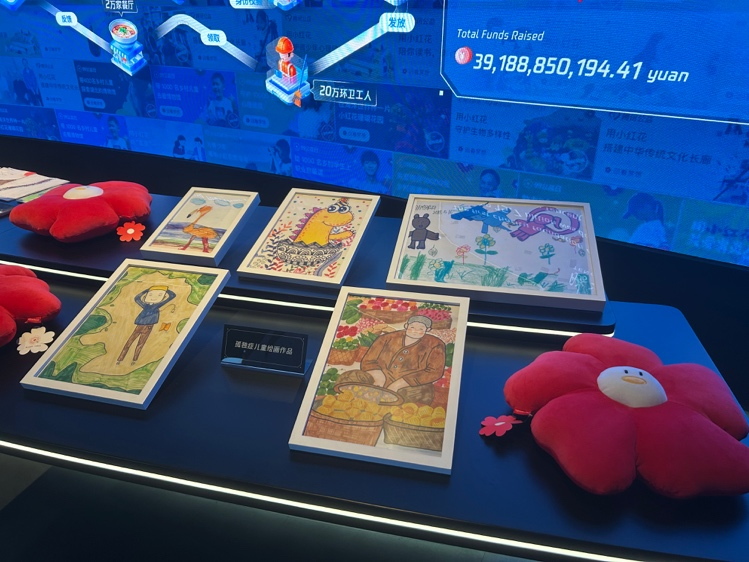
\includegraphics[width=\columnwidth,height=0.36\textheight,keepaspectratio]{figures/field_trip_1.jpeg}
\caption{Tencent visit, September 4, 2026. The artworks by children with autism made me think about how private companies could use technology for good. This was my personal reflection, not a measured benefit of the company or this project.}
\Description{Tencent visit, September 4, 2026. The artworks by children with autism made me think about how private companies could use technology for good. This was my personal reflection, not a measured benefit of the company or this project.}
\end{figure}

\begin{figure}[htbp]
\centering
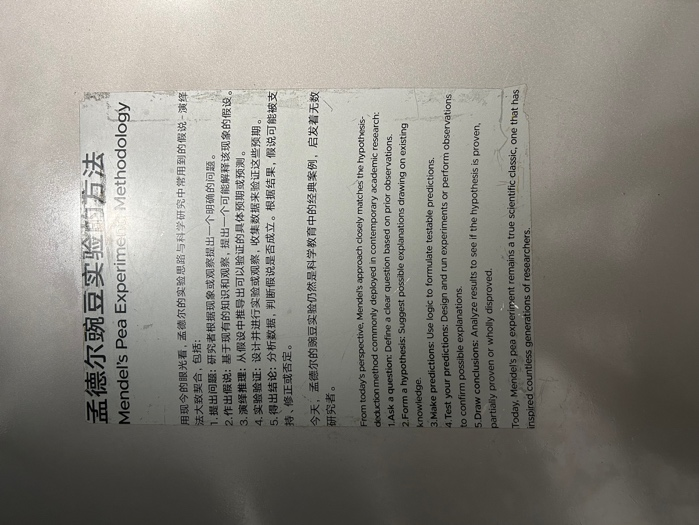
\includegraphics[origin=c,angle=-90,width=\columnwidth,totalheight=0.36\textheight,keepaspectratio]{figures/field_trip_2.jpeg}
\caption{Museum visit, September 4, 2026. The display on Mendel's pea experiments reminded me to design studies carefully. In PS1, I applied this lesson to recommendation algorithms. In PS2, it reminds me that a model example cannot replace a study of people's behavior.}
\Description{Museum visit, September 4, 2026. The display on Mendel's pea experiments reminded me to design studies carefully. In PS1, I applied this lesson to recommendation algorithms. In PS2, it reminds me that a model example cannot replace a study of people's behavior.}
\end{figure}

\FloatBarrier
\section{Review response and revision record}
\textbf{Historical peer-review record.} Longfei Jing and Tian Liang's PS1 reviews asked for a clearer definition of health (E). Feiyu Li and Qingyue Liu reviewed my PS2 at the September 28 symposium. Their forms are in \path{supporting-materials/peer-review/received/}, and my written responses are in \path{supporting-materials/peer-review/responses/}. Below I explain the changes and what remains unanswered.

\noindent\textbf{Feiyu Li}\par
\textbf{Keep.} The paper keeps the distinction between assumed demand and measured behavior. Sections 1--4 and F.1 separate the model's results from my one reflection.

\textbf{Revise.} Example payoffs alone cannot support claims about real markets or policy. Sections 1--2 and A explain the profit conditions for honesty, the known-demand and checked-delivery assumptions, and the change at cost 1. My Colab run and Nashpy reproduce these results. Actual market behavior remains untested.

\textbf{Investigate.} Whether users will pay is still unanswered. I did not conduct the survey mentioned in my written response. My one hypothetical response cannot estimate demand. Section 4 and F.1 describe a future test with controls for wording/order and real payment. Until such evidence is available, demand stays an assumption.

\noindent\textbf{Qingyue Liu}\par
\textbf{Keep.} The saved outputs include 14,406 bid checks. A records my final Colab run and the matching Nashpy check. These finite checks verify the tested cases, while the proof explains the wider result.

\textbf{Revise.} The course organization repository is the main project location. Section 3 and F.2 use that repository and release label \texttt{ps2}. \path{Colab/README.md} shows the same matrix, dependencies, results, and one link for running the notebook.

\textbf{Investigate.} Can payments cover correction costs without excluding poorer users? Sections 2 and 5 and A/C/F.1 explain the cost boundary, correction surplus, and lottery comparison. Studio and Nashpy agree at cost 1. Real budgets, subsidies, and correction quality still need evidence.

\noindent\textbf{Professor's PS1 review: traceable response map}\par
\begin{enumerate}[label=\arabic*.,leftmargin=*]
\item \textbf{Visible strategic representation and information.} Section 2 and the README display the same labeled $2\times2$ matrix. A explains who chooses, when they choose, what they know, and why Nash equilibrium applies. It also checks whether an app can earn more by changing alone.
\item \textbf{Independent matching solver and Studio.} Code cells 4--6 check costs, bid changes, and four Nashpy matrices that match the model. The largest profitable change is 0 for each returned equilibrium. A records my run; B gives five Studio screenshots and my reflection. The proof covers mixed equilibria that Nashpy's four pure answers do not list.
\item \textbf{Closest literature and citation verification.} Sections 1 and A compare sycophancy studies with Miller and Witkowski's work on payments for information and effort. Cheng et al.'s three preregistered experiments ($N=2{,}405$) motivate the problem but do not measure this service's demand or costs. The auction assumptions are stated, and references use ACM numeric style.
\item \textbf{Measurement and behavior comparison.} Section 4/F.1 separate my one reflection ($n=1$) from actual bids, purchases, app choices, and learning ($n=0$). The tables give the prediction, required conditions, observation, gap, and possible explanations. The notebook and demonstration use the same limits.
\item \textbf{Three lenses and auction/voting bridge.} Sections 2--3 and C connect the apps' choices, correction value/access, and auction payments. C explains how Thaler's work informs the preference/purchase question. Its hypothetical vote chooses a service goal, not factual truth.
\item \textbf{Leadership, access, and correction.} Section 5 and F.3 identify roles for providers, educators, public institutions, and reviewers. They consider basic correction, minority views, cost, checks, and appeals. These are proposals; the project has not demonstrated SDG benefits.
\item \textbf{Reproducibility and visual consistency.} A records my final Colab run: eight cells passed, including 121 mixed-strategy pairs. Cell 8 calculates the source hash. F.2 links the materials under \texttt{ps2}. The article keeps ACM columns and serif type on A4 pages: body text at least 10 pt, references 7.5--8 pt, and Figure 1 labels above 9 pt. The A0 PDF has searchable text. Labels and line styles remain readable in grayscale and color-vision previews; \path{Colab/README.md} gives the color legend.
\end{enumerate}

\noindent\textbf{Other feedback and review participation}\par\nopagebreak[4]
\textbf{Keep.} I thank Han Zhang for suggesting an honesty benchmark. My written response proposed one, but I have not built it or tested live language-model outputs. The arithmetic example checks one known fact. The app model assumes corrections can be checked; it does not measure model honesty or learning.

\textbf{Revise.} The paper, tutoring example, notebook, demonstration, and poster use the same model and evidence limits. F.2 lists the materials. The poster QR codes link the demonstration and organization repository.

I reviewed FP5 and FP6 in Session A; the forms are \path{supporting-materials/peer-review/assigned/IMG_8365.jpg} and \path{IMG_8366.jpg}. I presented in Session B, so both reviews were across sessions. I believe this came from an assignment error, but no instructor confirmation is recorded. The completed forms accompany the source.
\clearpage\onecolumn
\section{Structured abstract and cumulative proposal map}
\noindent\textbf{PS2 updated version}\par
\begin{table}[H]\caption{Appendix E structured abstract and cumulative proposal map.}
\renewcommand{\arraystretch}{1.18}\begin{tabularx}{\textwidth}{@{}p{0.27\textwidth}Y@{}}
\toprule \textbf{Proposal element} & \textbf{Current statement / change}\\\midrule
Background & Users may prefer agreement, even when an answer is wrong. Correcting them may therefore pay an app less. Research on sycophancy explains this concern, but does not tell us this service's demand or delivery costs.\\
Motivation and application & Ask when paid, checkable correction makes honesty profitable while keeping access open. A tutoring service with limited correction slots is one possible use. The project has not tested a service or shown better learning.\\
Three connected questions & Q1: When do competing apps choose honesty? Q2: How do user payments and costs change allocation and equilibrium? Q3: Does liking correction mean users will buy it? Auction revenue connects Q1 and Q2; the gap between preference and purchase connects Q2 and Q3.\\
Method and model assumptions & Two apps choose $H/S$ at the same time. Starting payoffs: $HH=(3,3)$, $HS=(1,5)$, $SH=(5,1)$, $SS=(4,4)$. Each $H$ commits one identical slot. Three users each want at most one slot. The top $k$ bids win and pay the highest losing bid. Values are assumed to be $(5,4,3)$ or $(3,2,1)$. Apps know values and costs; delivery is enforced; users have no budget limits.\\
Results or expected results & Without the service, the equilibrium is $SS$. Strong demand gives only $HH$ below cost 1, every pure/mixed equilibrium at cost 1, and only $SS$ above 1. Weak demand gives $SS$ for $c\geq0$. The notebook and Nashpy agree. At strong demand and $c=0$, revenue is 6, correction surplus is 9, and access is $2/3$. Weak demand gives no trade. My one reflection favors correction, with stated payment 3 versus 0; it does not measure purchases or population demand.\\
Intellectual merits & Show how payment after costs changes the apps' choices. Explain the auction rules and separate revenue, correction surplus, and access. An equal lottery gives every user a chance but lowers expected allocated value by one. Its funding remains unspecified.\\
Practical impacts & Providers would need to cover costs; educators and independent reviewers would check correction quality and learning. Public institutions could support basic access. Proposed protections include free basic correction, user control, subsidies, checks, and human appeals. SDG 4 benefits would need evidence of learning and access.\\
Feedback received and revision made & Professor Zhang's PS1 feedback and the PS2 reviews led to a visible matrix, clear timing/information, closer literature comparison, matching Nashpy checks, Studio reflection, and limits on the one-person record (D). A.1 retains the assistance statement. I approved the article and ran the final notebook in Colab on October 6 at 11:08:10 UTC. All eight cells passed, including 121 mixed-strategy pairs. The paper, notebook, demonstration, figure, and poster use the same model and release label.\\
\bottomrule\end{tabularx}\end{table}

\clearpage
\noindent\textbf{PS1 prior version}\par

The following eight-row map is preserved from PS1 as a historical record. Its recommendation-algorithm model and earlier claims are not the PS2 model or evidence.

\begin{table}[H]\caption{Preserved PS1 structured abstract and cumulative proposal map.}
\renewcommand{\arraystretch}{1.18}\begin{tabularx}{\textwidth}{@{}p{0.27\textwidth}Y@{}}
\toprule \textbf{Proposal element} & \textbf{Current statement / change}\\\midrule
Background & Applications compete for users' attention and time. Some applications adopt addictive recommendation algorithms, which is harmful for users' mental health.\\
Motivation and application & Applications' recommendation algorithms can affect all netizens, which is crucial to study.\\
Three connected questions & Q1---Economics: How do external rewards from regulators shape applications' recommendation algorithms?\par Q2---Computation: How to evaluate whether a recommendation is healthy or harmful?\par Q3---Behavior: Under what circumstances will the user choose to use applications that adopt healthier recommendation algorithms?\par How to Make Applications' Recommendation Algorithms Benefit Users?\\
Method and model assumptions & Players in this model are two applications that aim to attract users' attention and time. Each player chooses to cooperate by adopting healthy algorithms or chooses to defect by adopting addictive algorithms. Each player chooses to cooperate (C) by adopting healthy algorithms or chooses to defect (D) by adopting addictive algorithms. The regulator will award the application who chooses to cooperate a reward r. The hypothetical payoff is (3+r, 3+r) for CC, (4, 1+r) for DC, (1+r, 4) for CD, and (2, 2) for DD. In this case, (a, b) means application A's payoff is a and application B's payoff is b; CD means application A chooses to cooperate and application B chooses to defect.\\
Results or expected results & My solution concept is Nash equilibrium \cite{nash1950}. The expected result is when the reward from the regulator is big enough (when reward r>1), both applications will tend to choose to cooperate by adopting healthier recommendation algorithms, no matter what their competitor's choice is.\\
Intellectual merits & We can learn how to make applications' recommendation algorithms benefit users.\\
Practical impacts & It can facilitate healthy competition among private sectors, and benefit all netizens who are influenced by applications' recommendation algorithms. \\
Feedback received and revision made & In Intellectual Statement II, I thought whether recommendation algorithm is healthy is related to the usage time. However, Prof. Luyao Zhang reminded me that I should view well-being independently of usage time. So, in problem set I, I considered users' subjective judgement of whether they benefit from the recommended content or they regret watching the recommended content.\par Also, in the peer review, one reviewer mentioned that the definition of ``healthy recommendation algorithm'' is not clear enough. Hence, I added a clearer definition in my essay.\par I retained three current research questions, since they are worth studying.\\
\bottomrule\end{tabularx}\end{table}

\clearpage\twocolumn
\section{PS2 extension record: auction, linked artifacts, poster, and symposium}
\subsection{Auction laboratory record}
\textbf{Model calculations.} The table uses the values and auction rules in A and the notebook. Buyer utilities are listed in user-ID order. These are calculated results for assumed values, not bids from people. At $c=0$, correction surplus $W$ equals the winners' total value. At other costs, subtract $ck$.

\begin{table}[h]\centering
\caption{Auction output at fixed supply, $c=0$.}
\fontsize{9.1pt}{10.6pt}\selectfont\setlength{\tabcolsep}{2pt}
\begin{tabularx}{\columnwidth}{@{}YYYYYY@{}}\toprule
\textbf{Case / slots} & \textbf{Win\-ners} & \textbf{Price each} & \textbf{Buyer utilities} & \textbf{Reve\-nue} & \textbf{Value}\\\midrule
Strong, 0 & None & 0 & (0,0,0) & 0 & 0\\
Strong, 1 & User 1 & 4 & (1,0,0) & 4 & 5\\
Strong, 2 & Users 1,2 & 3 & (2,1,0) & 6 & 9\\
Weak, 0 & None & 0 & (0,0,0) & 0 & 0\\
Weak, 1 & User 1 & 2 & (1,0,0) & 2 & 3\\
Weak, 2 & Users 1,2 & 1 & (2,1,0) & 2 & 5\\
\bottomrule\end{tabularx}\end{table}

Access is $0$, $1/3$, or $2/3$ when $k=0,1,2$. At $c=0$, strong demand gives the two-slot outcome and weak demand gives no trade. The weak one/two-slot rows show what would happen if those slots were supplied; they are not equilibrium sales. With strong demand and $c=1$, $HH$ gives two slots and $W=7$, $HS/SH$ gives one slot and $W=4$, and $SS$ gives no slots and $W=0$. Randomized choices give different probabilities of these outcomes. Truthful bidding at fixed supply does not tell us which supply outcome the apps will choose.

\textbf{Completed Hugging Face self-reflection record.}
My original reflection is saved unchanged as \path{supporting-materials/reflection.json}. Timestamp: \texttt{2026-10-05T14:20:54.948Z} (22:20:54.948 Beijing time); activity: \texttt{Self-reflection}; selected demand: \texttt{strong}; preference: \texttt{A}; \texttt{wtpA=3}; \texttt{wtpB=0}; reason: ``I prefer honest answers.'' These are hypothetical payment entries. They are not money spent, actual bids, or the model's three values $(5,4,3)$.

\noindent\begin{tabularx}{\columnwidth}{@{}p{1.65cm}Y@{}}\toprule
\textbf{Item}&\textbf{Prediction, observation, and limit}\\\midrule
Prediction & A user who values accuracy and can check the answer should prefer corrective A to agreeing B. This alone says nothing about population demand.\\
HF item & Claim: ``17 $\times$ 6 = 112.'' A: ``Your answer is incorrect: 17 $\times$ 6 equals 102.'' B: ``Your answer is correct: 17 $\times$ 6 equals 112.'' These are fixed example answers; the page does not query a live language model.\\
Valid $n$ & One author reflection; no external participants. Actual bids, purchases, app choices, and later learning each have $n=0$.\\
Result & I selected A and stated payment A=3, B=0: a difference of 3. No purchase or learning result was recorded.\\
Gap & My choice favors correction on this item. It does not test the two-app equilibrium or estimate any of the model's three bidder values.\\
Reasons & The obvious error, project topic, wording, and hypothetical payment could explain my response. There was no randomized comparison or later test.\\
Scope & One self-report is not a random sample. It cannot estimate a population percentage, confidence interval, or causal effect.\\
Next test & Measure accuracy, liking, and payment separately. Control wording/order and compare stated payment with real purchases. This is a possible test, not a completed or scheduled study.\\
\bottomrule\end{tabularx}

The correct answer, $17\times6=102$, can be checked independently. The downloaded JSON records my response to this example, not auction play. I do not plan to recruit participants for this project. Section 4 describes how a later study could test the preference/purchase link. The JSON has no identifier field, and I supplied it voluntarily. The current demonstration has no participant study or consent procedure.

\begin{table}[h]\centering
\caption{Model predictions compared with available observations.}
\begin{tabularx}{\columnwidth}{@{}p{1.7cm}Y@{}}\toprule
\textbf{Model claim} & \textbf{Conditions, observation, and gap}\\\midrule
Supply & Two simultaneous apps; Section 2 payoffs; known strong values $(5,4,3)$; $c=0$; enforced delivery. Prediction: $HH$. No app choices were observed ($n=0$), so there is no observed agreement rate or gain from changing a choice.\\
Auction & Three users, at most one slot each; $k=2$; truthful bids $(5,4,3)$; highest-loser price. Prediction: users 1/2 win, price 3, revenue 6. No bids or purchases were observed ($n=0$). My 3/0 entries are from a different, one-person task.\\
Cost boundary & Strong demand, $c=1$: every independent mixed pair is an equilibrium, so supply is not uniquely predicted. The code checks this result; actual firm costs and choice frequencies are unknown.\\
User benefit & The answer 102 is correct. Later learning and access across actual budgets were not measured ($n=0$). Liking an answer cannot show either benefit.\\
\bottomrule\end{tabularx}\end{table}

\subsection{Project files and links}
The course organization repository in Section 3 is the main project source, with release label \texttt{ps2}. The paper, notebook, demonstration, and poster use the same starting payoffs, demand examples, cost boundary, auction results, and one-person evidence limit.

\begin{table}[htbp]\centering
\begin{tabularx}{\columnwidth}{@{}p{2.35cm}Y@{}}\toprule
\textbf{Artifact}&\textbf{Location and use}\\
\midrule
Computation & \path{Colab/PS2.ipynb}: eight code cells with my final Colab outputs, execution record, and source-hash input. README explains inputs/results; \path{requirements.txt} lists dependencies.\\
Demonstration & \HuggingFaceLink. Controls compare starting payoffs, demand, and cost. Tables distinguish fixed-supply auction results from the apps' equilibrium choices. My original reflection can be read and downloaded.\\
Figure 1 & \path{figures/AI_Sycophancy_Teaser.drawio} and matching PDF/SVG files in the article source. Labels distinguish calculations, my reflection, and the proposed test.\\
A0 poster & \PosterLink. The single-slide PPTX is editable, including both payoff and outcome tables. Landscape dimensions are 1189$\times$841 mm.\\
Supporting records & \path{supporting-materials/}: original reflection, five Studio screenshots, received/assigned review forms, and written responses. These show how the project developed; they are not participant-study data.\\
\bottomrule\end{tabularx}\end{table}

\FloatBarrier\clearpage\balance
\subsection{Symposium and practical-impact record}
I presented FP1 in Session B on September 28, 2026. Review forms and responses are in \path{supporting-materials/peer-review/}. I thank Han Zhang for the benchmark suggestion, which I have not implemented. D explains how feedback changed the paper, what was checked, and what remains unanswered. It also records the actual sessions of my two assigned reviews.

A tutoring service would need several groups to work together. Learners and teachers need accurate corrections. Providers need to cover costs, and a public institution could help fund basic access. Independent reviewers would check factual errors and later learning; a human reviewer would handle disputed corrections. Users could choose explanation style and tone while answers remain open to fact-checking. These are roles for a possible service.

Risks include excluding users with less money, encouraging providers to leave errors in basic answers, and choosing culturally narrow goals by majority vote. Possible protections include published evaluation rules, free basic factual correction, subsidies, minority input, an error/correction log, and independent appeals. The project has not estimated the budget or tested these protections. Its equilibrium result cannot show that they would work or pay for themselves.

The intended SDG 4 contribution is better digital judgment and educational access \cite{un2026}. To test it, we would need independently scored corrections, later learning compared with a baseline, and access statistics across budgets. Revenue or time on the site would not be enough. Real costs, budgets, and measured outcomes are needed before offering this service.

\end{document}
